\documentclass{egee}
%\usepackage{doxygen}

\usepackage{xspace}
%\usepackage{doxygen}

\def\LB{L\&B\xspace}
\def\JP{JP\xspace}
%\def\eg{e.\,g.}
\def\eg{for example\xspace}
\def\Eg{For example\xspace}
%\def\ie{i.\,e.}
\def\ie{that is\xspace}
\def\wrt{with respect to\xspace}
\def\Dash{---\penalty-1000}

\long\def\TODO#1{\par\noindent\textbf{TODO:} {\sl#1}\par}
\long\def\ludek#1{}

\hyphenation{plug-in}


\title{Job Provenance}
\Subtitle{Administrator's Guide}
\author{CESNET EGEE II JRA1 team}
\DocIdentifier{EGEE-II....}
\Date{\today}
\Activity{JRA1: Middleware Engineering and Integration}
\DocStatus{DRAFT}
\Dissemination{PUBLIC}
\DocumentLink{http://...}

\Abstract{ This administrator's guide explains how to administer the Job
Provenance (\JP) service. Several deployment scenarios are described together
with the installation, configuration, running and troubleshooting steps. }

\begin{document}

\begin{center}
{\bf Delivery Slip}
\end{center}
\begin{tabularx}{\textwidth}{|l|l|l|X|X|}
\hline
           & {\bf Name} & {\bf Partner} & {\bf Date} & {\bf Signature} \\
\hline
{\bf From} &                  &  & & \\
\hline
{\bf Reviewed by} & &  & & \\

\hline
{\bf Approved by} & & & & \\
\hline
\end{tabularx}

\begin{center}
{\bf Document Change Log}
\end{center}

\begin{tabularx}{\textwidth}{|l|l|X|X|}
\hline
{\bf Issue } & {\bf Date  } & {\bf Comment } & {\bf Author  } \\   \hline

\hline
\end{tabularx}

\begin{center}
{\bf Document Change Record}
\end{center}

\begin{tabularx}{\textwidth}{|l|l|X|}
\hline
{\bf Issue } & {\bf Item  } & {\bf Reason for Change } \\   \hline

\hline
\end{tabularx}

%
% Official text received on October 6, 2004
%
\vfill{\bf Copyright }\copyright{\bf Members of the EGEE Collaboration. 2004. 
See http://eu-egee.org/partners for details on the copyright holders. 

EGEE (``Enabling Grids for E-science in Europe'') is a project funded by
the European Union.  For more information on the project, its partners
and contributors please see http://www.eu-egee.org.

You are permitted to copy and distribute verbatim copies of this
document containing this copyright notice, but modifying this document
is not allowed. You are permitted to copy this document in whole or in
part into other documents if you attach the following reference to the
copied elements: ``Copyright }\copyright{\bf 2004. Members of the EGEE
Collaboration. http://www.eu-egee.org''

The information contained in this document represents the views of
EGEE as of the date they are published. EGEE does not guarantee that
any information contained herein is error-free, or up to date.

EGEE MAKES NO WARRANTIES, EXPRESS, IMPLIED, OR STATUTORY, BY
PUBLISHING THIS DOCUMENT.}


\clearpage

\newpage
\tableofcontents

\newpage
\section{Introduction}
\TODO{Do a reasonable merge with the JPUG-Introduction, do not duplicate text...}


\subsection{Job Provenance service overview}
The information about jobs submitted to gLite Workload Management
System is collected by the Logging and Bookkeeping (LB) service.
LB tracks jobs in terms of events and processes them in
a~real time to give overall view on the actual job state. The user may
query the bookkeeping server to obtain either the raw events or the
computed job state, she may also register for receiving notifications
on particular job state changes.

While the LB is intended to keep track of jobs during its lifetime, it
is not supposed to be used for long term archival of such data. The
Job Provenance (JP) service is designed to provide long-term storage
of all data related to job life and allow the end user to perform
data-mining in this data.
The JP is supposed to provide the permanent storage of
the job related information as stored within the \LB, to couple it with
the input sandboxes and other system oriented information necessary to
reproduce the environment where a~particular job run.

\subsubsection{Gathering data into Job Provenance}
Fig.~\ref{fig:psinter} depicts basic gLite middleware components and
their interaction with the Job Provenance.

\begin{figure}[htpb]
  \centering
  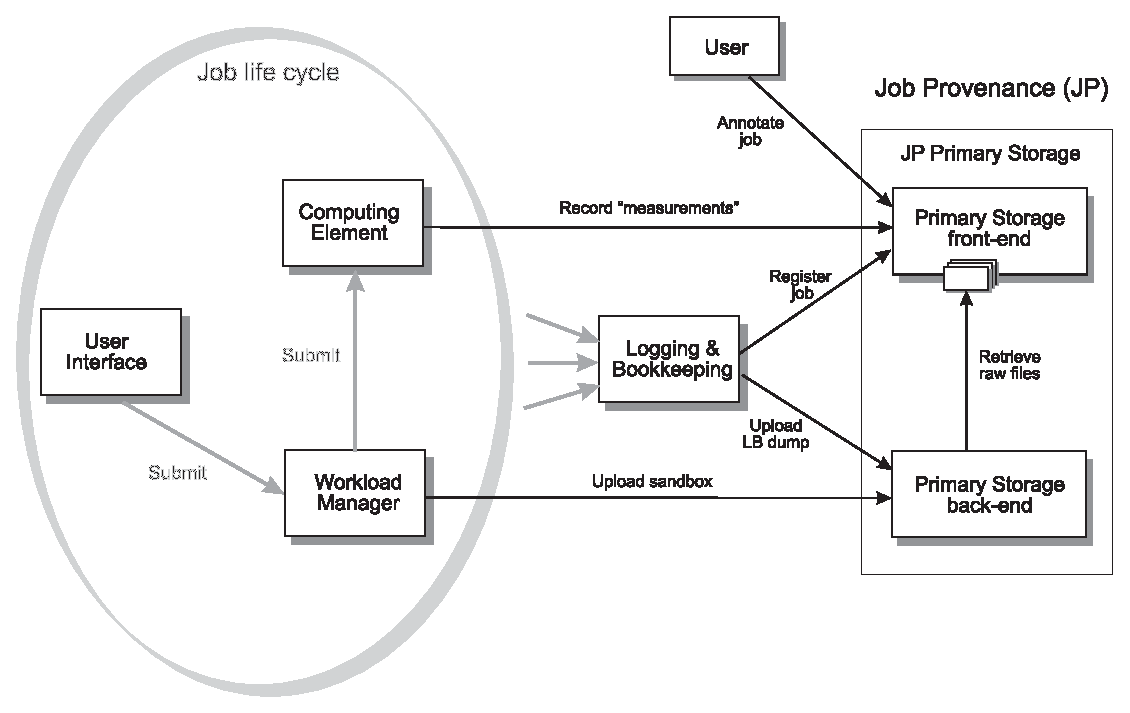
\includegraphics[scale=0.7]{JP-interactions}
  \caption{Data flow into gLite Job Provenance}
  \label{fig:psinter}
\end{figure}

JP is formed of two classes of services: permanent \emph{Primary
Storage} (JPPS) accepts and stores job data while possibly volatile
and configurable \emph{Index Servers} (JPIS) provide an optimized
querying and data-mining interface to the end-users.  The only direct
data retrieval scenario supported by JPPS is the case when user know exact ID
of jobs in the interest.

\subsubsection{Getting data from Job Provenance}

The role of \emph{Index Servers} (JPIS) is processing and re-arranging the data
from Primary Storage(s) into a~form suitable for frequent and complex user
queries. A user query part of JP is shown in Fig.~\ref{fig:query}.

\begin{figure}[htpb]
  \centering
  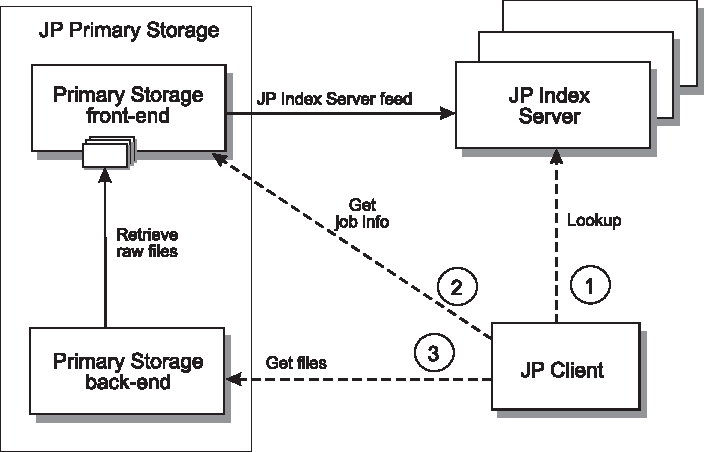
\includegraphics[scale=0.8]{JP-query}
  \caption{Index Server interactions}
  \label{fig:query}
\end{figure}

Index Servers are created, configured, and populated semi-dynamically
according to particular user community needs.  It is responsibility of
its administrator to setup the JPIS with appropriate configuration. There
is no prescribed relationship between Primary Storage and Index Server
installations.  An Index Server may retrieve data from multiple
Primary Storages and vice versa.

% TODO: update 
% The interface exposed by JPIS to the end user is described in the
% chapter~\ref{reference}. Command line interface tool for end-user
% interface to the JPIS is described in the chapter~\ref{CLI}.  See the
% next chapter (use cases) for futher description of JP to user
% interactions.


% LB-JP-interaction
\subsection{Interaction with Logging and Bookeeping (\LB)}

In this section we describe the interaction of JP with Logging and Bookkeeping
(\LB) service.  The data flows between LB and JP services are displayed in
Figure~\ref{fig:LB-JP-interactions}.  These flows are numbered and one can use
this numbers to find additional information about each flow in
table~\ref{tab:LB-JP-interactions}.

\begin{figure}[htpb]
  \centering
  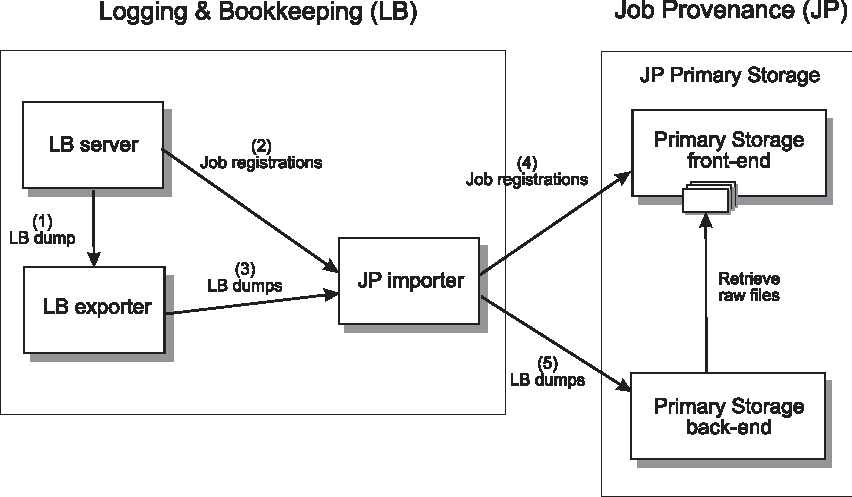
\includegraphics[width=0.9\hsize]{LB-JP-interaction-details}
  \caption{LB to JP interactions detail overview}
  \label{fig:LB-JP-interactions}
\end{figure}

\begin{table}[htpb]
 \centering
  \begin{tabular}{|c|p{3cm}|l|p{9cm}|}
    \hline
    &spool directory&initiated by&description\\
    \hline
    \hline
    1&lb.export.dump,
      lb.export.dump.keep&lb-exporter&
      Export of LB job records into spool directory. It uses glite-lb-purge utility. LB-exporter reads this spool directory in a regular manner and implement next processing of LB dumps. Optionally it can keep handled dumps in lb.export.dump.keep.\\
    \hline
    2&lb.export.jpreg&LB server&When new job come to the LB server 
    it stores its
    registration into the spool directory. It is responsibility of
    JP-importer process to handle such registrations.\\
    \hline
    3&lb.export.jpdump,
      lb.export.jobs,
      lb.export.jobs.keep&lb-exporter&
      LB-exporter do its processing of LB dumps (they are in per job form) and passes on it to the JP-importer using the spool directory lb.export.jpdump and temporary storage lb.export.jobs. It can keep the job files for futher usage.\\
    \hline
    4&none&jp-importer&JP importer handles registrations received from LB
    server and sends it to the JP primary server front-end (using its WS
    interface).\\
    \hline
    5&none&jp-importer&JP importer handles LB dumps received from LB
    exporter and sends it to the JP primary server back-end using its
    gridftp interface.\\
    \hline
  \end{tabular}
  \caption{LB to JP data flows description}
  \label{tab:LB-JP-interactions}
\end{table}


Notes:
\begin{itemize}
 \item Only JP Primary Storage (JPPS) server is involved in described
   data flows. JP Index Servers are not part of this picture (they are
   feeded via corresponding JPPS).
 \item Only flows number 4 and 5 are designed to be inter-host. All
   the other interactions assume the components are on the same host and
   do use access to a shared filesystem.
 \item Data flow number 1 use glite-lb-purge utility (see its
   documentation) and passes to it argument from lb.export.purgeargs
   clause of the deployment configuration file. This argument contain
   the timeouts controlling after how long period of time a job
   staying in a terminal state is to be purged from the LB server.
 \item The LB exporter have a feature to store LB job event dumps in a
   directory for further handling (e.g. for job statistic tool). This behaviour
   is controled by lb.export.jobs.keep deployment config file clause (leave
   this clause empty if you don't use dumps for futher handling).
 \item The LB exporter also have a feature to keep all handled LB
   dumps (in glite-lb-purge format) in filesystem. This feature is
   controlled by lb.export.dump.keep.
 \item LB exporter is not a deamon, it's periodic invocation is
   provided by cron deamon.
\end{itemize}



%
\subsection{Deployment scenarios}



\newpage
\section{Installation}
\TODO{}

\subsection{Complete RPMs description}
\subsection{Daemons description}
\subsection{CLI tools description}



\newpage
\section{Configuration}
\TODO{}

\subsection{JPPS}
\subsubsection{Setting up the MySQL database}


\subsection{JPIS}

\begin{alltt}
The JP-IS server daemon assume prior creation of its database. Simple tool
  for database creation is org.glite.jp.index/config/dbsetup.sh

customize startup script /etc/init.d/glite-jp-indexd (see below)
  and set up service startup using this script


Currently, configuration is done by command line options,  and
some hard-coded options.


The index server takes the following options:

./glite-jp-indexd [option]
        -d, --debug      don't run as daemon, additional diagnostics
        -q, --query-type hist/cont/both (default history)
        -n, --noauth     don't check user identity with result owner
        -m, --mysql      database connect string
        -p, --port       port to listen
        -i, --pidfile    file to store master pid
        -o, --logfile    file to store logs
        -x, --config     file with server configuration

The config file parameter is required. There is the example configuration in
$GLITE_LOCATION/etc/glite-jpis-config.xml.
\end{alltt}


\newpage
\section{Running and stopping the services}
\TODO{}

\subsection{Tests if everything works properly}



\newpage
\section{Testing JP functionality}
% AKA Testplan

\def\req{\noindent\textbf{Prerequisities: }}
\def\how{\noindent\textbf{How to run: }}
\def\result{\noindent\textbf{Expected result: }}
\def\jpps{\noindent\textbf{JP PS log should contain: }}
\def\jpis{\noindent\textbf{JP IS log should contain: }}


\subsection{JPPS standalone tests}

\subsubsection{Job registration}

\paragraph{Basic functionality}
\label{regjob}
\req\ Running JPPS

\how
\begin{itemize}
\item call RegisterJob operation:
\begin{verbatim}
$ jpps-test RegisterJob JOBID OWNER
\end{verbatim}
where JOBID and OWNER should be replaced with real values, JOBID should not have
been registered with JP before.

\item  call GetJobAttributes to verify:
\begin{verbatim}
$ jpps-test GetJobAttr JOBID http://egee.cesnet.cz/en/Schema/JP/System:owner
\end{verbatim}
\end{itemize}
\result Should print the OWNER value supplied.

\paragraph{AuthZ check}
\req\ JPPS running, a~job registered with the procedure in~\ref{regjob}

\how\ 
Call GetJobAttributes using different user credentials 

\result\ 
Should fail with ``Permission denied'' error

\subsubsection{Tag recording}
\label{tagreg}

\paragraph{Basic functionality}
\req\
JPPS running, a~job registered with the procedure in~\ref{regjob}

\how 
\begin{itemize}
\item Call RecordTag operation:
\begin{verbatim}
$ jpps-test  RecordTag JOBID TAGNAME STRINGVALUE
\end{verbatim}
\item Call GetJobAttributes to verify
\begin{verbatim}
$ jpps-test  GetJobAttr JOBID TAGNAME
\end{verbatim}
\end{itemize}
\result
The recorded value should be returned.

\how\ Record another values(s) of the same tag by repeating the RecordTag call

\result\ GetJobAttr should return all the recorded values


\paragraph{AuthZ check}
\req\ JPPS running, a~job registered with the procedure in~\ref{tagreg} \\
\how\ Call RecordTag using different user credentials \\
\result\ Should fail with ``Permission denied'' error \\


\subsubsection{File upload}


\paragraph{Basic functionality}
\req\ JPPS running, my certificate subject amont JPPS trusted peers, 
\verb'globus-url-copy' in PATH

\how
Run the aggregate test script from \verb'org.glite.jp.primary/build'

\begin{verbatim}
$ ../examples/jpps_store_test -o 'OWNER' -d ../examples/job_template
\end{verbatim}
(substitute real cert.\ subject for OWNER)

\result\ 
The script calls JPPS operations RegisterJob and StartUpload, 
uploads an \LB\ job log generated from the template file,
calls CommitUpload.

Finally, the upload is checked by retrieving two attribute
values: LB/Attributes:user and LB/Attributes:finalStatusk via the GetJobAttr
call. 
Both calls should return OK and print reasonable values.

%- call StartUpload, LB dump file type
%* check with GetJobFiles -- shoud return nothing
%- upload via ftp
%- call CommitUpload
%* check with GetJobFiles -- should return URL
%- retrieve and check the file

\paragraph{Phase checks}
\TODO{salvet}
% soubor nelze zapsat pred otevrenim operaci StartUpload
% nelze cist pred Commitem
% nelze zapsat po Commitu

\paragraph{AuthZ checks}
(should fail)

\TODO{salvet}
%* call GetJobFiles with different credentials
%
%* StartUpload with different credentials
%
%- StartUpload
%* ftp upload with different credentials
%
%* ftp GET with different credentials


\paragraph{Cleanup}
(Foreseen test for feature which is not implemented yet)
%- call StartUpload, short timeout
%- upload via ftp
%(don't call CommitUpload)
%* uploaded file should be purged after timeout

\subsection{\LB\ plugin}
%\TODO{honik}
\LB\ plugin is a component integrating the \LB\ functionality into JP.


\subsubsection{Standalone tests}
\LB\ plugin as a standalone component is used for example in the \texttt{glite-lb-statistics} 
program (part of org.glite.lb.utils). This program reads a dump file of events related to
one particular job and using the \LB\ plugin it computes the job state and many other job 
statistics. See the \LB\ testplan for more details.

\subsubsection{Integrated tests}
\req JPPS running with the \texttt{-P/path/to/the/glite\_lb\_plugin.so}

\how 
\begin{itemize}
\item call GetJobAttributes to get the LB attributes
\begin{verbatim}
$ jpps-test GetJobAttr JOBID ATTRIBUTE

where ATTRIBUTE is one of the 
http://egee.cesnet.cz/en/Schema/LB/Attributes:jobId
http://egee.cesnet.cz/en/Schema/LB/Attributes:user
http://egee.cesnet.cz/en/Schema/LB/Attributes:VO
http://egee.cesnet.cz/en/Schema/LB/Attributes:eNodes
http://egee.cesnet.cz/en/Schema/LB/Attributes:eProc
http://egee.cesnet.cz/en/Schema/LB/Attributes:RB
http://egee.cesnet.cz/en/Schema/LB/Attributes:CE
http://egee.cesnet.cz/en/Schema/LB/Attributes:host
http://egee.cesnet.cz/en/Schema/LB/Attributes:UIHost
http://egee.cesnet.cz/en/Schema/LB/Attributes:CPUTime
http://egee.cesnet.cz/en/Schema/LB/Attributes:finalStatus
http://egee.cesnet.cz/en/Schema/LB/Attributes:finalStatusDate
http://egee.cesnet.cz/en/Schema/LB/Attributes:finalStatusReason
http://egee.cesnet.cz/en/Schema/LB/Attributes:LRMSDoneStatus
http://egee.cesnet.cz/en/Schema/LB/Attributes:LRMSStatusReason
http://egee.cesnet.cz/en/Schema/LB/Attributes:retryCount
http://egee.cesnet.cz/en/Schema/LB/Attributes:additionalReason
http://egee.cesnet.cz/en/Schema/LB/Attributes:jobType
http://egee.cesnet.cz/en/Schema/LB/Attributes:nsubjobs
http://egee.cesnet.cz/en/Schema/LB/Attributes:lastStatusHistory
http://egee.cesnet.cz/en/Schema/LB/Attributes:fullStatusHistory
\end{verbatim}
\end{itemize}

\result Should print the corresponding LB attributes

\subsection{JPPS-JPIS interaction (feeds)}


%set of queries (how many?) with different "triggering conditions":
%- on job registration
%- on LB file upload
%- on RecordTag

%corresponding sets of jobs to each query, each containing jobs which match
%and which don't

%- initial IS release -- single query, so just one set of jobs
%- due to 3.2 no point in pre-loading PS database, use 1.3.1

\subsubsection{Batch feed}
%- upload jobs to PS
%- start feed
%* check IS contents (jobs and expected attr values)

\req\ Clean JP-PS and JP-IS database.

\how\
\begin{enumerate}
 \item \emph{Start JP primary server}
 \item \emph{Register job to PS}
  \begin{alltt}
     for j in `seq 1 10`;  
     do  
        for i in glite-jp-primary-sample_job*.lb; 
        do 
            ./glite-jp-primary-store-test -o  \emph{CERT_DN} 
                -t "my_tag=car" -s https://localhost:8901 -d $i; 
        done; 
     done
  \end{alltt}
  You should see something like:
  \begin{alltt}
    ** ./glite-jp-primary-test -s https://localhost:8901 RegisterJob
    https://nonexistent.test.server/jpps_store_test_7199
           /O=CESNET/O=Masaryk University/CN=Milos Mulac
    OK
    ** ./glite-jp-primary-test -s https://localhost:8901 GetJobAttr
    https://nonexistent.test.server/jpps_store_test_7199
           http://egee.cesnet.cz/en/Schema/JP/System:owner
    OK
    Attribute values: /O=CESNET/O=Masaryk University/CN=Milos Mulac
           SYSTEM  Thu Feb 16 14:40:02 2006
    ....
    Attribute values:
           car     FILE    Thu Feb 16 14:40:02 2006
  \end{alltt}
 \item \emph{Start JP index server, using history query}\\
 \item \emph{Check content of IS database}\\
  \begin{alltt}
   mysql -u jpis -e "select * from jobs;" jpis
  \end{alltt}
 You should get 50 results, similar to:
  \begin{alltt}
| jobid                            | dg_jobid
| ownerid                          | aclid | ps
+----------------------------------+---------------------------------+
| 7bd73b18b33410ba605fba99dbdd803f | https://nonexistent.test.server/jpps_store_test_5993
| 5864429d57da18e4ecf9ea366c6b2c9c | NULL  | https://localhost:18950 |
...
50 rows in set (0.00 sec)
  \end{alltt}
\end{enumerate}
\result{} Expected results in the IS database content check (last step).


\subsubsection{Incremental feed - simple tests}
%- register feed
%- upload job to PS 
%* check PS and IS output

\req\ Clean JP-PS and JP-IS database.

\how\
\begin{enumerate}
 \item \emph{Start JP primary server}
 \item \emph{Start JP index server, using continuous query}
 \item \emph{Registerjob}
  \begin{alltt}
	./jpps-test -s https://localhost:18950 RegisterJob 
	https://nonexistent.test.server/jpps_store_test_6880 "/O=CESNET/O=Masaryk 
	University/CN=Milos Mulac"
	OK
  \end{alltt}
  \jpps\
  \begin{alltt}
	[22004] client DN: /O=CESNET/O=Masaryk University/CN=Milos Mulac
	__jpsrv__RegisterJob https://nonexistent.test.server/jpps_store_test_6881 
	/O=CESNET/O=Masaryk University/CN=Milos Mulac
	feed to https://scientific.civ.zcu.cz:8902, job https://nonexistent.test.server/
	jpps_store_test_6881
  \end{alltt}
  \jpis\
  \begin{alltt}
	...
	[21984] incoming request
	__jpsrv__UpdateJobs
	...
	glite_jpis_lazyInsertJob: owner '/O=CESNET/O=Masaryk University/CN=Milos Mulac'
	found
	glite_jpis_insertAttrVal: (http://egee.cesnet.cz/en/Schema/JP/System:owner) 
	sql=INSERT INTO attr_52942b8c70bab8491ab5d3b9713d79f5 (jobid, value, full_value, 
	origin) VALUES (
        '6e436919404778b75cd27eef266190bb',
        'S:/O=CESNET/O=Masaryk University/CN=Milos Mulac',
        'S:/O=CESNET/O=Masaryk University/CN=Milos Mulac',
        '1'
)
	glite_jpis_insertAttrVal: (http://egee.cesnet.cz/en/Schema/JP/System:regtime) ...
	...
  \end{alltt}

 \item \emph{Start upload}
  \begin{alltt}
	./jpps-test -s https://localhost:18950 StartUpload 
	https://nonexistent.test.server/jpps_store_test_6880 
	urn:org.glite.jp.primary:lb 1234 text/plain
	OK
	Destination: gsiftp://scientific.civ.zcu.cz:8960//home/mulac/jp/internal/
	data/5864429d57da18e4ecf9ea366c6b2c9c/1889/jpps_store_test_6880/lb
	Commit before: Sat Mar 17 10:12:48 2007
  \end{alltt}
  \jpps\
  \begin{alltt}
	[22004] client DN: /O=CESNET/O=Masaryk University/CN=Milos Mulac
	data_basename: (null)
  \end{alltt}
  \jpis\
	nothing
 \item \emph{globus-url-copy}
  \begin{alltt}
	globus-url-copy file:/home/mulac/src/ORG/org.glite.jp.primary/build/job.6880
	gsiftp://scientific.civ.zcu.cz:8960//home/mulac/jp/internal/
	data/5864429d57da18e4ecf9ea366c6b2c9c/1889/jpps_store_test_6880/lb
  \end{alltt}
  \jpps\
	nothing \\
  \jpis\
	nothing \\
  \noindent\textbf{Other:}
	File specified in gsiftp URL should be created.
 \item \emph{Commit upload}
  \begin{alltt}
	./jpps-test -s https://localhost:18950 CommitUpload 
	gsiftp://scientific.civ.zcu.cz:8960//home/mulac/jp/internal/data/
	5864429d57da18e4ecf9ea366c6b2c9c/1889/jpps_store_test_6880/lb
	OK
  \end{alltt}
  \jpps\
  \begin{alltt}
	[22004] client DN: /O=CESNET/O=Masaryk University/CN=Milos Mulac
	glite_jpps_match_file: https://nonexistent.test.server/jpps_store_test_6880 lb (null)
	lb_plugin: opened 8 events
	lb_plugin: close OK
	feed to https://scientific.civ.zcu.cz:8902, job https://nonexistent.test.server/
	jpps_store_test_6880
  \end{alltt}
  \jpis\
  \begin{alltt}
	...
	__jpsrv__UpdateJobs
	...
	glite_jpis_insertAttrVal: (http://egee.cesnet.cz/en/Schema/LB/Attributes:CE) 
	sql=INSERT INTO attr_c47f78255056386d2b3da6d506d1f244 (jobid, value, 
	full_value, origin) VALUES (
        '39a0a14f4fc084fbb466728986e5ea2f',
        'S:destination CE/queue',
        'S:destination CE/queue',
        '3'
	)
	...
  \end{alltt}
 \end{enumerate}

\result{} Expected results in logs.


\subsubsection{Incremental feed}
%- register feed
%- upload jobs to PS one by one
%* check IS contents (matching jobs should turn up, others not)

\req\ Clean JP-PS and JP-IS database.

\how\
\begin{enumerate}
 \item \emph{Start JP primary server}
 \item \emph{Start JP index server, using continuous query}
 \item \emph{Register job to PS}
  The same as in previous test case.

 \item \emph{Check output of IS}\\
  You should see incomming connection logs, and among them
  several times something like:
  \begin{alltt}
    
   INSERT INTO attr_52942b8c70bab8491ab5d3b9713d79f5 (jobid, value,
                                        full_value, origin) VALUES (
     '6f4866f3e4f8204c269449e6924d73c0',
     'S:/O=CESNET/O=Masaryk University/CN=Milos Mulac',
     'S:/O=CESNET/O=Masaryk University/CN=Milos Mulac',
     '1')
   ....
  \end{alltt}
 \item \emph{Check content of IS database}\\
 Do the same test as in previous test case. It must give you the same
 result. You can also look whether the insert from previous step was 
 successful:
 \begin{alltt}
  mysql -u jpis -e "select * from
    attr_52942b8c70bab8491ab5d3b9713d79f5;" jpis
 \end{alltt}
  should return:
 \begin{alltt}
| jobid                            | value
| full_value                                      | origin |
+----------------------------------+-----------------------------------+
| 76698aabbf5d60dfa5b42c279e1f0e8c | S:/O=CESNET/O=Masaryk University/CN=Milos
Mulac 
| S:/O=CESNET/O=Masaryk University/CN=Milos Mulac |      1 |
 \end{alltt}
\end{enumerate}
\result{} Expected database INSERTs in the JP-IS (last two steps).

\subsubsection{Multiple feeds at time}
\TODO{TBD}

\subsubsection{Advanced feed features (to be implemented)}
- remove (not implemented in PS yet)
- splitted info about one job (check that the PS doesn't duplicate
  attribute values) - probably covered in 3.2


\subsubsection{PS-IS AuthZ}
\TODO{Not implemented yet}

\subsection{IS queries}


%TBD: insert job sets via JP-IS interaction or directly?
%        - better to populate database directly, independent on previous chain
%
%All basic tests:
%- clear IS database
%- insert prepared job set
%- ask queries and check answers
%- clear database
%
%TBD: Is one job set enough?
%        - better to have one complete set
%

A majority of test from this chapter is automated by shell
script. The script is located in \texttt{org.glite.jp.index} module
under \texttt{example/query-tests} directory and called \texttt{run-test.sh}.
It is available as a part of JP index server RPM package.

\begin{hints}
The testing shell script is highly configurable via
environmental varibles.  Please, run the script (run-test.sh) with
'-?' option to get list of all variables and their meaning, if you are
not satisfied with default setting.
\end{hints}

\subsubsection{Simple query}
This test starts new index server instance, creates testing DB
and populate it with prepared data sample. Then simple query is given
to server, answer is checked with supposed return output and
cleanup is done.


\how\ Run \texttt{run-test.sh}

\begin{hints} 
The query is in file test/simple\_query.in and has following
  form: (status=Ready)
\end{hints}

\subsubsection{Complex query test}
This is similar to simple query test, only tested query is more complicated.

\how\ Run \texttt{run-test.sh}

\begin{hints}
The query is in file test/complex\_query.in and has followhing
  form: (status=Done OR status=READY) AND (user!=God)
\end{hints}

\subsubsection{Feed \& query test}
This test starts testing index server, feeds it by
mimicing bahaviour of primary storage server by sending data
via soap call, and then asks the index server using a complex
query. After that it checks the responce and does cleanup.

More precise description of steps:
\begin{enumerate}
 \item Simulation of response from a primary storage, making appropriate
   changes in JP-IS database (inserts feedid).
 \item Invocation of updateJobs wsdl call, normally invoked by JP-PS, and
   sending this way some data to the JP-IS which stores them in its database.
 \item Invocation of queryJobs wsdl call, normally called by user
   program, obtaining previously inserted data. Test query used here has form
   (status=Done OR status=Ready) AND (user!=God).
\end{enumerate}

\how\ Run \texttt{run-test.sh}

\subsubsection{AuthZ checks}
This test verifies that qeury responses are properly restricted by
authorization checks. Currently only implicit ACLs are implemented
inside JP-IS server, so explicit ACLs and its evaluation is to be implemented.

There are 3 scenarios to be verified:
\begin{itemize}
 \item Authorization (checking ownership) is swithed off (IS with -n
   option). This scenario is tested by simple query test described above.
 \item Only user jobs are returned and jobs not owned by the user posing
   the query are not covered by the query response. This scenario is
   covered by Feed \& query test described above.
 \item Check that queries to jobs not owned by the IS user are
   returning empty response. The same behaviour as simple query test
   described above but with user credential not matching job
   owner. This test is implemented by \texttt{run-test.sh} under AuthZ
   check part.
\end{itemize}

\subsubsection{Another supposed tests not implemented yet}

\begin{itemize}
 \item Check "origin" behaviour -- queries with origin tag
 \item IS CLI tests -- use prepared config files and command line parameters
  and check expected QueryJobs contents
\end{itemize}


\subsection{IS standalone advanced features}
\TODO{Not implemented yet}

\subsubsection{Server startup}

\paragraph{Reboot persistency / configuration vs. database content}
    situations handling
- prepared config files
- checking behaviour (how?) after reboot with different config file

\paragraph{Registration of PS feeds}
! already covered by 3
- prepared config files
- checking appropriate FeedIndex calls

\subsubsection{Admin interface}
\TODO{Admin interface not implemented yet}

\subsubsection{Type plugin}
\TODO{type plugin tests -- to be designed, future type plugin implementation}

\subsection{Deployment}
\TODO{tests on JP deployment process}
\TODO{TBD}



\newpage
\section{Troubleshooting}
\TODO{}

\subsection{Debugging}
\subsection{Fine tuning the performance}



\nocite{jgc}
\bibliographystyle{unsrt}
\bibliography{lbjp}

\end{document}
